\documentclass{article}

\usepackage[letterpaper,top=3cm,bottom=2cm,left=3cm,right=3cm,marginparwidth=1.75cm]{geometry}

\usepackage{amsmath}
\usepackage{amssymb}
\usepackage{graphicx}
\usepackage{float}
\usepackage{algpseudocode}
\usepackage{multicol}

\title{CPSC 322 Introduction to AI}
\author{Kaitian Xie}
\date{May 11, 2019}

\graphicspath{ {./images/} }

\begin{document}

\maketitle
\pagebreak

\section{Introduction}

\section{Search}

\subsection{Intro to Search}
% TODO

\subsubsection{Directed Acyclic Graph (DAG)}

\begin{itemize}
    \item \textbf{Directed ayclic graph}: a graph with no cycles and where the arcs have associated directions.
\end{itemize}

\subsubsection{Search with Costs}

\begin{itemize}
    \item \textbf{Cost of a path}: sum of costs of its arcs $cost(<n_0, \ldots, n_k>) = \sum\limits_{i=1}^{k} (<n_{i-1}, n_i>)$
    \item \textbf{Optimal solution}: solution with minimal cost.
\end{itemize}

\subsubsection{Heuristic}

\begin{itemize}
    \item \textbf{Search heuristic ($h(n)$)}: an estimate of the cost of the lowest-cost path from node $n$ to a goal node.
    \item \textbf{Admissible heuristic}: $h(n)$ is admissible if it is never an overestimate, i.e. $h(n)$ is a lower bound. To construct an admissible heuristic, we can either:
    \begin{itemize}
        \item drop some constraints or
        \item make less restrictions on actions
    \end{itemize}
    \item \textbf{Dominance}: If $h_2(n) \geq h_1(n)$ for every state $n$ (both admissible), then $h_2$ dominates $h_1$.
    \item we can combine two admissible heuristic functions: $h(n) = max\{h_1(n), h_2(n)\}$.
\end{itemize}

\subsubsection{Uninformed Search vs Heuristic Search}

\begin{itemize}
    \item \textbf{Uninformed}: not taking the goal into account until the goal state is reached.
    \item \textbf{Heuristic}: there exists extra knowledge to guide the search.
\end{itemize}

\subsection{Generic Search Algorithm}

\begin{algorithmic}
    \Require{a graph, a start node $n_0$, $goal(n)$}
    \State{$frontier := [<n_0>]$}
    \While{$frontier$ is not empty}
        \State{Select and remove a path $<n_0, \ldots, n_k>$ from $frontier$}
        \If{$goal(n_k)$}
            \State{return $<n_0, \ldots, n_k>$}
        \EndIf
        \For{every neighbor $n$ of $n_k$}
            \State{Add $<n_0, \ldots, n_k, n>$ to $frontier$}
        \EndFor
    \EndWhile
\end{algorithmic}

\begin{figure}[H]
    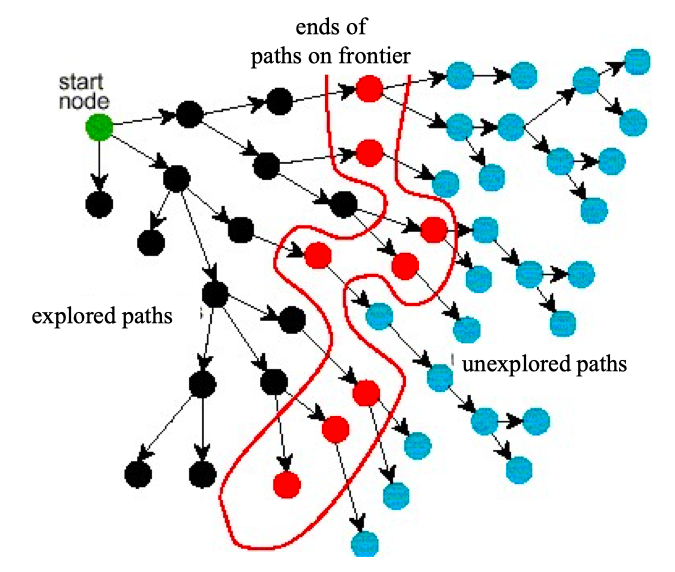
\includegraphics[width=\textwidth]{generic_search_algo_visualization}
    \centering
\end{figure}

\subsubsection{Branching Factor ($b$)}

\begin{itemize}
    \item \textbf{Forward branching factor}: number of arcs going out of a node
    \item \textbf{Backward branching factor}: number of arcs going into a node
\end{itemize}

\subsubsection{Complete \& Optimal}

\begin{itemize}
    \item \textbf{Complete}: can find a solution.
    \item \textbf{Optimal}: can find the best solution.
\end{itemize}

\subsubsection{Complexity}

\begin{itemize}
    \item \textbf{Time complexity}: amount of time needed in the worst-case scenario; expressed in terms of maximum path length ($m$) and maximum branching factor ($b$).
    \item \textbf{Space complexity}: amount of space needed in the worst-case scenario; expressed in terms of $m$ \& $b$.
\end{itemize}

\subsection{Depth-First Search (DFS)}

\begin{itemize}
    \item $frontier$ is a stack $[p_1, p_2, \ldots, p_k]$
    \item neighbors of last node of $p_1$ are $\{n_1, \ldots, n_k\}$
    \item
    \begin{algorithmic}
        \While{$frontier$ is not empty}
            \State{$p := frontier.pop()$}
            \State{$n_{end} := $ last node of $p$}
            \If{$goal(n_{end})$}
                \State{Return $p$}
            \EndIf
            \State{$frontier.push((p, n_1), \ldots, (p, n_k))$}
        \EndWhile
    \end{algorithmic}
    \item not complete because DFS may get ``stuck'' in a graph that has cycles.
    \item not optimal because DFS may return a longer solution while a shorter solution exists
    \item time complexity: $O(b^m)$
    \item space complexity: $O(bm)$
    \item DFS is appropriate when:
        \begin{itemize}
            \item space is restricted.
            \item there are many solutions, perhaps with long path solutions, particularly for the case in which all paths lead to a solution.
        \end{itemize}
    \item DFS is inappropriate when:
        \begin{itemize}
            \item cycles
            \item shallow solution
            \item optimality is needed
        \end{itemize}
\end{itemize}

\subsection{Breadth-First Search}

\begin{itemize}
    \item $frontier$ is a queue $[p_1, p_2, \ldots, p_k]$
    \item neighbors of last node of $p_1$ are $\{n_1, \ldots, n_k\}$.
    \item
    \begin{algorithmic}
        \While{$frontier$ is not empty}
            \State{$p := frontier.poll()$}
            \State{$n_{end} := $ last node of $p$}
            \If{$goal(n_{end})$}
                \State{Return $p$}
            \EndIf
            \State{$frontier.offer((p, n_1), \ldots, (p, n_k))$}
        \EndWhile
    \end{algorithmic}
    \item complete because it doesn't get stuck in cycles
    \item optimal because it guarantees to find the path that involves the fewest paths
    \item time complexity: $O(b^m)$
    \item space complexity: $O(b^m)$
\end{itemize}

\subsection{Iterative Deepening Search}

\begin{itemize}
    \item
        \begin{itemize}
            \item Look with DFS for solution at depths $1, 2, \ldots$
            \item If a solution can't be found at depth $D$, try again at depth $D+1$
            \item depth-bounded depth-first searcher
            \item given a bound $B$, assume the paths of length $B$ can't be expanded.
        \end{itemize}
    \item time complexity: $O(b^m)$

    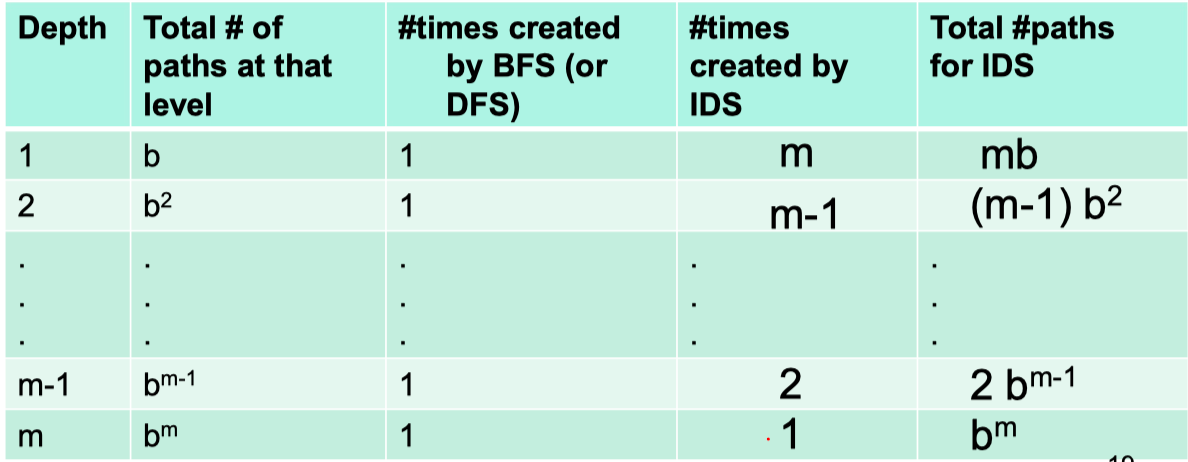
\includegraphics[scale=0.3]{ids_time_complexity}
    
    \begin{align*}
        b^m  + 2b^{m-1} + 3b^{m-2} + \ldots + mb 
        &= b^m (1 + 2b^{-1} + 3b^{-2} + \ldots + mb^{1-m}) \\
        & \leq b^m \sum\limits_{i=1}^{\infty} ib^{1-i} \\
        &= b^m (\frac{b}{b-1})^2 \\
        &= O(b^m)
    \end{align*}
\end{itemize}

\subsection{Lowest-Cost-First Search (LCFS)}

\begin{itemize}
    \item
    \begin{itemize}
        \item Select a path with the lowest cost from $frontier$ (a priority queue).
        \item not complete if there exists a cycle with zero or negative arc costs, otherwise it is complete
        \item not optimal if negative costs exist, otherwise it is optimal
        \item time complexity: $O(b^m)$
        \item space complexity: $O(b^m)$
            \begin{itemize}
                \item costs are equal $\Rightarrow$ BFS
            \end{itemize}
    \end{itemize}
\end{itemize}

\subsection{Best-First Search}

\begin{itemize}
    \item Select a path from the $frontier$ with minimal h-value (for the end node).
    \item The $frontier$ is implemented by a priority queue order by h-value.
    \item This is a greedy approach since it always takes a locally best path.
    \item not complete: if there exist low h-values in a cycle, BestFS gets stuck.
    \item not optimal: a heuristic might be misleading.
    \item time complexity: $O(b^m)$
    \item space complexity: $O(b^m)$
    \item BestFS is appropriate when:
        \begin{itemize}
            \item $h(n)$ is very good.
        \end{itemize}
\end{itemize}

\subsection{$A^{*}$}

\begin{itemize}
    \item LCFS + BestFS
    \item $f(p) = cost(p) + h(p)$
    \item The $frontier$ is implemented by a priority queue ordered by f-value.
    \item $A^{*}$ always selects a path that has the lowest estimated total distance to a goal.
    \item complete: $a^{*}$ always tests shorter underestimate of the total cost, so not missing anything
    \item optimal: $A^{*}$ is optimal if:
        \begin{itemize}
            \item $b$ is finite
            \item costs are strictly positive
            \item $h(n)$ is non-negative and admissible
        \end{itemize}
    \item proof of optimality: \textit{Lecture 8 slides 24-32}
    \item optimal efficiency: among all optimal algorithms that start from the same start node and use the same heuristic, $A^{*}$ expands the minimal number of paths.
\end{itemize}

\subsection{Branch-and-Bound Search (B\&B)}

\begin{itemize}
    \item $frontier$ implemented a stack, similar to DFS
    \item order of adding neighbours can be customized
    \item keeps track of a lower bound and an upper bound on a each path:
        \begin{itemize}
            \item lower bound: $LB(p) = f(p) = cost(p) + h(p)$
            \item upper bound: $UB = \text{cost of the best solution found so far}$ (initialize $UB = \infty$)
        \end{itemize}
    \item when a path $p$ is selected for expansion
        \begin{itemize}
            \item if $LB \geq UB$: remove $p$ from $frontier$
            \item else expand $p$
        \end{itemize}
    \item not complete: B\&B gets stuck in a graph with cycles
    \item optimal, but not optimal efficient
    \item time complexity: $O(b^m)$
    \item space complexity: $O(mb)$ (like DFS)
\end{itemize}

\subsection{Iterative Deepening $A^{*}$ ($IDA^{*}$)}

\begin{itemize}
    \item search depth-first, but to a fixed depth/bound
    \item depth measured in f-values
    \item if you don't find a solution, update the bound with the lowest f-value that passed the previous bound
    \item time complexity: $O(b^m)$
    \item space complexity: $O(mb)$
\end{itemize}

\subsection{Memory-Bounded $A^{*}$ ($MBA^{*}$)}

\begin{itemize}
    \item keep $frontier$ in memory as we can
    \item if we need to free some memory, we delete:
        \begin{itemize}
            \item the worst paths (with highest f-values)
            \item ``back them up'' to a common ancestor
            \item update $h(n)$ of the ancestor if possible
        \end{itemize}
\end{itemize}

\subsection{Summary of Search Strategies}

\begin{figure}[H]
    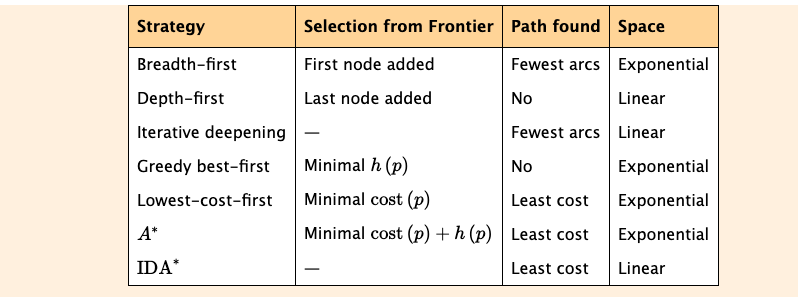
\includegraphics[width=\textwidth]{summary_of_search_strategies}
    \centering
\end{figure}

\subsection{Cycle Checking}

\begin{itemize}
    \item Prune a path that ends in a node already on the path
    \item Pruning doesn't remove an optimal solution.
    \item linear time complexity
\end{itemize}

\subsection{Multiple-Path Pruning}

\begin{itemize}
    \item Prune a path to node $n$ that you already found a path to.
\end{itemize}

\section{CSP}

\subsection{Variables/Features, Domains, and Possible Worlds}

\begin{itemize}
    \item Capital letters to represent variables.
    \item \textbf{Domain}: $dom(V)$ = possible values for $V$.
    \item \textbf{Possible world}: a complete assignment of values to a set of variables.
\end{itemize}

\subsection{Constraints}

\begin{itemize}
    \item \textbf{Constraint}: restrictions on the values for one or more variables.
        \begin{itemize}
            \item function that returns true when given values for each variable satisfy the constraint
            \item list of valid domain values for each variable participating in the constraint
        \end{itemize}
    \item \textbf{Unary constraint}: restriction involving a single variable.
    \item \textbf{K-ary constraint}: restriction involving the domains of $k$ different variables.
\end{itemize}

\subsection{Constraint Satisfaction Problems (CSP)}

\begin{itemize}
    \item \textbf{Constraint satisfaction problem} consists of:
    \begin{itemize}
        \item a set of variables
        \item a domain for each variable
        \item a set of constraints
    \end{itemize}
    \item \textbf{Model} is an assignment of values to variables (i.e. possible world) that satisfies all of the constraints.
\end{itemize}

\subsection{Generate-and-Test Algorithm}

\begin{algorithmic}
    \For{$a$ in $domA$}
        \For{$b$ in $domB$}
            \For{$c$ in $domC$}
                \If{$abc$ satisfies all constraints}
                    \State \Return{$abc$}
                \EndIf
            \EndFor
        \EndFor
    \EndFor
    \State \Return {$NULL$}
\end{algorithmic}

\begin{itemize}
    \item can solve any CSP
    \item bad runtime
\end{itemize}

\subsection{CSPs as Search Problems}

\begin{itemize}
    \item \textbf{States}: assignments of values to a subset of the variables.
    \item \textbf{Start state}: the empty assignment.
    \item \textbf{Neighbours}: nodes in which values are assigned to one additional variable.
    \item \textbf{Goal(n)}: set of constraints
    \item \textbf{Goal state}: a state which assigns a value to each variable, and satisfies all of the constraints.
    \item \textbf{Solution}: possible world that satisfies the constraints.
    \item \textit{Note}: 
        \begin{itemize}
            \item Path is unimportant.
            \item depth = num of variables
            \item $h(n)$ is useless since all solutions have the same distance from the goal
            \item The tree is finite and has no cycles.
        \end{itemize}
    \item We use \underline{DFS} as our search strategy.
    \item Pruning: if an end node violates one or more constraints, we a solution cannot exist beyond that node $\Rightarrow$ remove that path.
\end{itemize}

\subsection{Consistency}

\begin{itemize}
    \item Prune domains before searching.
    \item \textbf{Domain consistency}: a variable is domain consistent if no value of its domain is ruled impossible by any unary constraint.
    \item \textbf{Constraint network}: a graph with
        \begin{itemize}
            \item one node for every variable
            \item one node for every constraint
            \item undirected edges between variable nodes and constraint nodes
        \end{itemize}
    \item \textbf{Arc consistency}: an arc $<x, r(x, y)>$ is consistent if for each value $x$ in $dom(X)$, there is some value $y$ in $dom(Y)$ such that $r(x, y)$ is satisfied. A network is arc consistent if all its arcs are consistent.
        \begin{itemize}
            \item To enforce arc consistency, we remove $x$ from $dom(X)$ is there is no value $dom(Y)$ to satisfy the constraint.
        \end{itemize}
\end{itemize}

\subsection{Arc Consistency Algorithm}

\begin{itemize}
    \item General idea:
        \begin{enumerate}
            \item Go through all the arcs.
            \item Make each arc consistent by pruning if needed.
            \item Reconsider consistent arcs that could be made inconsistent again by this pruning.
            \item Eventually reach a ``fixed point'': all arcs are consistent.
        \end{enumerate}
    \item Pseudo-code:
        \begin{algorithmic}
            \State{$TDA \gets \text{all arcs in Constraint Network}$}
            \While{$TDA$ is not empty}
                \State{Select an arc $a$ from $TDA$}
                \If{$a$ is not consistent}
                    \State{Make $a$ consistent}
                    \State{Add arcs to $TDA$ that may now be inconsistent}
                \EndIf
            \EndWhile
        \end{algorithmic}
    \item Detailed version:
        \begin{figure}[H]
            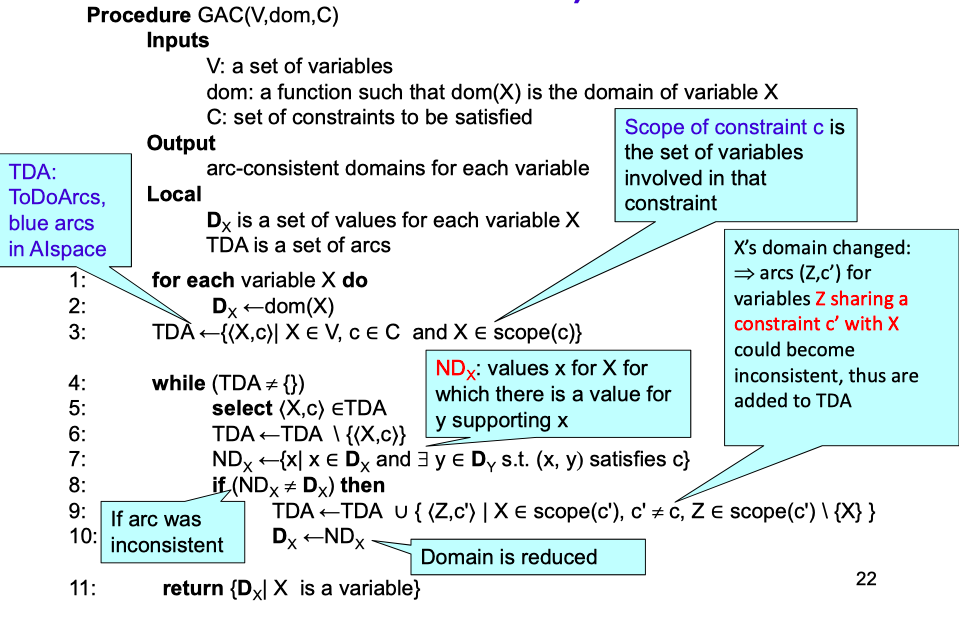
\includegraphics[width=\textwidth]{gac}
            \centering
        \end{figure}
    \item Complexity (Worst-case)
        \begin{itemize}
            \item $d = \text{max size of a variable domain}$
            \item $n = \text{number of variables}$
            \item Assume all constraints are binary.
            \item Max number of binary constraints = $\frac{n * (n - 1)}{2}$
            \item The same arc can be inserted in $TDA$ $d$ times.
            \item $d^2$ steps are involved in checking the consistency of an arc.
            \item Overall complexity: $O(n^2d^3)$, better than DFS.
        \end{itemize}
    \item Outcomes:
        \begin{enumerate}
            \item One domain is empty $\Rightarrow$ no solution.
            \item Each domain has a single value $\Rightarrow$ unique solution.
            \item Some domains have more than one value $\Rightarrow$ zero or more solutions.
                \begin{itemize}
                    \item Arc consistency is not good enough $\Rightarrow$ we still need to search.
                \end{itemize}
        \end{enumerate}
\end{itemize}

\subsection{Domain Splitting}

\begin{itemize}
    \item Split a problem in a number of disjoint cases, so $sol(CSP) = \bigcup\limits_{i} sol(CSP_i)$.
    \item By splitting, we may be able to run AC again. However, we need to keep all CSPs around.
    \item Arc consistency + domain splitting:
        \begin{itemize}
            \item \textbf{States}: $vector(D(V_1), \ldots, D(V_2))$ of remaining domains, with $D(V_i) \subseteq dom(V_i)$ for each $V_i$.
            \item \textbf{Start state}: vector of original domains $(dom(V_i), \ldots, dom(V_n))$
            \item \textbf{Successor function}: reduce one of the domains + run arc consistency
            \item \textbf{Goal state}: vector of unary domains that satisfy all constraints:
                \begin{itemize}
                    \item only one value left for each variable
                    \item assignment of each variable to its single value is a model
                \end{itemize}
            \item \textbf{Solution}: that assignment
        \end{itemize}
    \item \#CSPs to keep at a time: $O(bm)$
\end{itemize}

\subsection{Local Search}

\begin{itemize}
    \item general idea:
        \begin{enumerate}
            \item Start from a possible world.
            \item Generate some neighbors.
            \item Move from the current node to a neighbor.
        \end{enumerate}
    \item \textbf{CSP}: a set of variables, domains for these variables, and constraints on their joint values.
    \item \textbf{Node}: a complete assignment to all of the variables.
    \item \textbf{Neighbor relation}: specified by some small incremental change to the variable assignment.
    \item \textbf{Scoring function}: judges cost of a node (want to minimize).
    \item \textbf{Iterative best improvement}: selects the neighbor that optimizes some evaluation function (minimal number of constraint violations).
        \begin{itemize}
            \item \textbf{Evaluation function (h(n))}: number of constraint violations in state $n$.
            \item \textbf{Greedy descent}: evaluates $h(n)$ for each neighbor, picks the neighbor $n$ with minimal $h(n)$.
            \item \textbf{Hill climbing}: equivalent algorithm for maximization problems (maximizes the number of satisfied constraints).
        \end{itemize}
    \item
        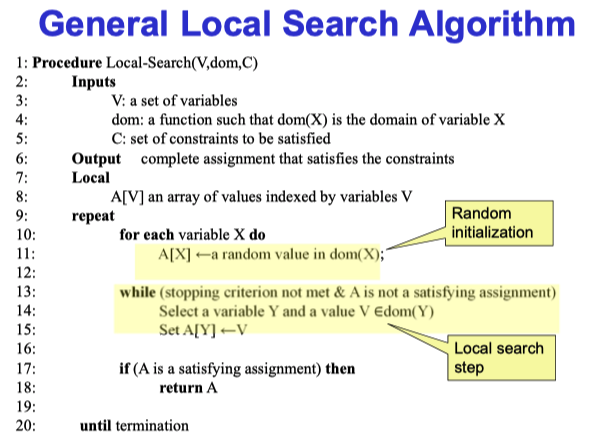
\includegraphics[scale=0.6]{general_local_search_algorithm}
    \item Most research in local search is about finding effective mechanisms for escaping from local minima. The iterative best improvement gets tapped in locally optimal minima.
\end{itemize}

\subsection{Stochastic Local Search (SLS)}

\begin{itemize}
    \item \textbf{Start node}: random assignment
    \item \textbf{Goal}: assignment with zero unsatisfied constraints
    \item \textbf{Heuristic function (h)}: \# unsatisfied constraints
    \begin{itemize}
        \item the lower, the better
    \end{itemize}
    \item SLS is a mix of 
    \begin{itemize}
        \item \textbf{Greedy descent}: move to a neighbor with lowest $h$
        \item \textbf{Random walk}: take some random steps, i.e. move to neighbor with some randomness
        \item \textbf{Random restart}: reassigning values to all variables
    \end{itemize}
\end{itemize}

\subsection{Greedy Descent vs Random Sampling}

\begin{itemize}
    \item \textbf{Greedy descent}:
        \begin{itemize}
            \item good for finding local minima
            \item bad for exploring new parts of the search space
        \end{itemize}
    \item \textbf{Random sampling}:
        \begin{itemize}
            \item good for exploring new parts of the search space
            \item bad for finding local minima
        \end{itemize}
\end{itemize}

\subsection{Selecting Neighbors}

\begin{itemize}
    \item \textbf{One stage selection}:
        \begin{itemize}
            \item the best neighbor
            \item a random variable-value pair
        \end{itemize}
    \item \textbf{Two state selection} (first select variable $V$, then new value for $V$):
        \begin{itemize}
            \item selecting variables:
                \begin{itemize}
                    \item the variable which participates in the largest number of conflicts
                    \item a random variable that participates in some conflict
                    \item a random variable
                \end{itemize}
            \item selecting rules:
                \begin{itemize}
                    \item the best value for the chosen variable
                    \item a random value for the chosen variable
                \end{itemize}
        \end{itemize}
\end{itemize}

\subsection{Comparing SLS Algorithms}

\begin{itemize}
    \item Time taken is a random variable.
    \item Runtime variations of 2 order of magnitude in repeated runs.
    \item Stagnation $\Rightarrow$ $\infty$ runtime
\end{itemize}

\subsection{SLS Variants}

\begin{itemize}
    \item \textbf{Simulated annealing}
        \begin{itemize}
            \item Key idea: Change the degree of randomness.
            \item Annealing: a metallurgical process where metals are heated and then slowly cooled.
                \begin{itemize}
                    \item starts with high tendency to take random steps.
                    \item over time, more likely to follow the scoring function.
                \end{itemize}
            \item Algorithm:
                \begin{itemize}
                    \item At the node $n$. Pick a variable at random and a new value at random. Generate $n'$.
                    \item if $n'$ is an improvement ($h(n) - h(n') > 0$, adopt it; otherwise, adopt it with a probability: $e = \frac{h(n) - h(n')}{T}$
                \end{itemize}
        \end{itemize}
    \item \textbf{Taboo Search}
        \begin{itemize}
            \item Make partial assignments as Taboo.
            \begin{itemize}
                \item stops repeatedly visiting the same (or similar) local minima.
            \end{itemize}
            \item A queue of $k$ variable-value pairs that are taboo.
                \begin{itemize}
                    \item $k$ needs to be optimized empirically.
                \end{itemize}
        \end{itemize}
    \item \textbf{Population Based SLS}
        \begin{itemize}
            \item Maintain a population of $k$ individuals
                \begin{itemize}
                    \item At every stage, update your population.
                    \item Whenever one individual is a solution, report it.
                \end{itemize}
        \end{itemize}
    \item \textbf{SLS for Constraint Optimization Problems}
        \begin{itemize}
            \item constraint optimization problems
                \begin{itemize}
                    \item hard constraints: need to satisfy all of them.
                    \item soft constraints: need to satisfy them as well as possible.
                    \item can have weighted constraints:
                        \begin{itemize}
                            \item minimize $h(n)$ = sum of weights of unsatisfied constraints in $n$.
                            \item hard constraints have large weights.
                            \item some soft constraints can be more important than other soft constraints $\Rightarrow$ larger weights.
                        \end{itemize}
                \end{itemize}
        \end{itemize}
\end{itemize}

\section{Planning}

\subsection{Intro to Planning}

\begin{itemize}
    \item \textbf{Planning}: build a sequence of actions that, if executed, takes the agent from the current state to a state that achieves a goal.
        \begin{itemize}
            \item actions = assignments of values to variables
            \item no notion of path to a solution: only final assignment matters.
        \end{itemize}
    \item A planning problem consists of
        \begin{itemize}
            \item goal
            \item description of states of the world
            \item description of available actions
                \begin{itemize}
                    \item when each action can be applied
                    \item what its effects are
                \end{itemize}
        \end{itemize}
    \item STRIPS representation:
        \begin{itemize}
            \item \textbf{Preconditions}: a set of assignments to features must be satisfied in order for the action to be applicable in a state.
            \item \textbf{Effects}: a set of assignments to features that are caused by the action.
        \end{itemize}
    \item A planning problem can be either a pure search problem/CSP problem.
\end{itemize}

\subsection{Forward Planning}

\begin{itemize}
    \item Search in the state-space graph:
        \begin{itemize}
            \item \textbf{States}: possible worlds.
            \item \textbf{Arcs}: possible actions in state $s$.
            \item \textbf{Plan}: a path from the initial state to a state that satisfies the goal.
        \end{itemize}
    \item Standard Search vs. Specific R\&R Systems
        \begin{multicols}{2}
            CSP
            \begin{itemize}
                \item \textbf{State}: assignments to a subset of the variables.
                \item \textbf{Successor function}: assign values to a ``free'' variable.
                \item \textbf{Goal test}: set of constraints.
                \item \textbf{Solution}: possible world that satisfies the constraints.
                \item \textbf{Heuristic funciton}: none (all solutions at the same distance from start)
            \end{itemize}
            
            \columnbreak
            
            Planning
            \begin{itemize}
                \item \textbf{State}: full assignments of values to features
                \item \textbf{Success function}: states reachable by applying actions with preconditions satisfied in the current state.
                \item \textbf{Goal test}: partial assignment of values to features.
                \item \textbf{Solution}: a sequence of actions.
                \item \textbf{Heuristic function}
            \end{itemize}
        \end{multicols}
        \item Heuristics for forward planning: number of actions needed to get from $s$ to goal.
            \begin{itemize}
                \item Count number of unsatisfied sub-goals (may not be admissible when an action can achieve multiple sub-goals).
                \item Plan by ignoring action preconditions.
            \end{itemize}
\end{itemize}

\subsection{Planning as CSP}

\begin{itemize}
    \item Action preconditions and effects are virtually constraints between:
        \begin{itemize}
            \item the action
            \item the states in which it can be applied
            \item the states that it generate
        \end{itemize}
    \item Make both states and actions into variables.
    \item The action constraints relate to states at a given time $t$, the corresponding valid actions and the resulting states at $t+1$ (as many as state and action variables as we have planning steps).
    \item \textbf{Horizon k}: ``unroll the plan'' for a fixed number of steps.
        \begin{itemize}
            \item Construct a CSP variable for each STRIPS state variable at each time step from 0 to $k$.
            \item Construct a boolean CSP variable for each STRIPS action at eacth time step form 0 to $k-1$.
        \end{itemize}
\end{itemize}

\section{Logic}

\subsection{Intro to Logic}

\begin{itemize}
    \item \textbf{Syntax}: specifies the symbols used, and how they can be combined to form legal sentences.
        \begin{itemize}
            \item knowledge base: set of sentences in the language
        \end{itemize}
    \item \textbf{Semantics}: specifies the meaning of symbols and sentences.
    \item \textbf{Reasoning theory/proof procedure}: a specification of how an answer can be produced
        \begin{itemize}
            \item \textbf{Sound}: only generates correct answers with respect to the semantics
            \item \textbf{Complete}: guaranteed to find an answer if it exists.
        \end{itemize}
\end{itemize}

\subsection{Propositional Definite Clause Logic (PDCL)}

\begin{itemize}
    \item \textbf{Atom}: symbol starting with a lower case letter.
    \item \textbf{Body}: 
        \begin{itemize}
            \item atom
            \item of the form $b_1 \wedge b_2$ ($b_1$ and $b_2$ are bodies)
        \end{itemize}
    \item \textbf{Definite clause}:
        \begin{itemize}
            \item atom
            \item rule of the form $h \leftarrow b$ ($h$ is an atom and $b$ is a body)
        \end{itemize}
    \item \textbf{Knowledge base (KB)}: set of definite clauses.
\end{itemize}

\subsection{Semantics}

\begin{itemize}
    \item Semantics allow you to relate the symbols in the logic to the domain you're trying to model.
    \item \textbf{Interpretation I} assigns a truth value to each atom.
    \item 
\end{itemize}

\subsection{Bottom-Up Proof Procedure}

\begin{itemize}
    \item proof procedure:
    \begin{algorithmic}
        \State{$C \gets \{\}$}
        \Repeat
            \State{Select clause $h \rightarrow b_1 \wedge \ldots \wedge b_m$ in $KB$ such that $b_i \in C$ for all $i$, and $h \notin C$}
            \State{$C \gets C \cup \{h\}$}
        \Until{no more clauses can be selected}
    \end{algorithmic}
    
    $KB \vdash G$ if $G \subseteq C$ at the end of this procedure ($C$ is a fixed point).
    \item 
    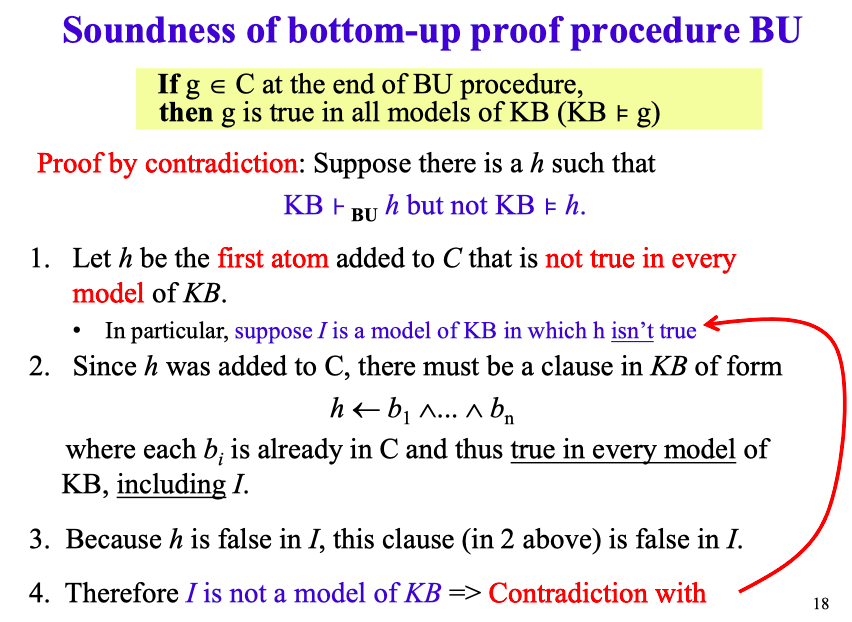
\includegraphics[scale=0.45]{soundness_of_bu}
    \item proof of completeness
        \begin{itemize}
            \item \textbf{Minimal model}: a specific interpretation of $KB$
                \begin{itemize}
                    \item every atom in $C$ at the end of BU is true
                    \item every other atom is false
                \end{itemize}
        \end{itemize}
\end{itemize}

\end{document}
